\documentclass{article} % For LaTeX2e
\usepackage{nips15submit_e,times}
\usepackage{hyperref}
\usepackage{url}
\usepackage{graphicx}
\usepackage{float}
\usepackage{amsmath}
\usepackage{multirow,array}
\usepackage{listings}
\usepackage{amsfonts}
\usepackage{caption}
\usepackage{subfigure}
\usepackage{algorithm,algorithmic}
%\usepackage[UTF8]{ctex} uncomment if needs Chinese support
%\usepackage{fontspec}

%\documentstyle[nips14submit_09,times,art10]{article} % For LaTeX 2.09

\renewcommand{\algorithmicrequire}{ \textbf{Input:}} %Use Input in the format of Algorithm
\renewcommand{\algorithmicensure}{ \textbf{Output:}} %UseOutput in the format of Algorithm

\definecolor{mygreen}{rgb}{0,0.6,0}
\definecolor{mygray}{rgb}{0.5,0.5,0.5}
\definecolor{mymauve}{rgb}{0.58,0,0.82}
\lstset{ %
backgroundcolor=\color{white},   % choose the background color
basicstyle=\footnotesize\ttfamily,        % size of fonts used for the code
columns=fullflexible,
breaklines=true,                 % automatic line breaking only at whitespace
captionpos=b,                    % sets the caption-position to bottom
tabsize=4,
commentstyle=\color{mygreen},    % comment style
escapeinside={\%*}{*)},          % if you want to add LaTeX within your code
keywordstyle=\color{blue},       % keyword style
stringstyle=\color{mymauve}\ttfamily,     % string literal style
frame=single,
rulesepcolor=\color{red!20!green!20!blue!20},
% identifierstyle=\color{red},
language=python,
numbers=left
}

\title{CS231 Course Report}


\author{
Liu Junnan
}

% The \author macro works with any number of authors. There are two commands
% used to separate the names and addresses of multiple authors: \And and \AND.
%
% Using \And between authors leaves it to \LaTeX{} to determine where to break
% the lines. Using \AND forces a linebreak at that point. So, if \LaTeX{}
% puts 3 of 4 authors names on the first line, and the last on the second
% line, try using \AND instead of \And before the third author name.

\newcommand{\fix}{\marginpar{FIX}}
\newcommand{\new}{\marginpar{NEW}}

%\nipsfinalcopy % Uncomment for camera-ready version

\begin{document}

\maketitle

\section{Introduction}
In the past weeks I got dived into CS231 course and learned fundamentals on deep learning and specifically computer vision, including both supervised and unsupervised learning. Besides three assignments related to the course are finished with great effort but all of them turn out to be extremely useful to help understanding the ideas and principles of machine learning algorithms. In this report I will make a brief conclusion on what I have learned from CS231 course.


\section{Supervised Learning Algorithms(Shallow, Classic)}
In supervised learning, some "shallow" algorithms, like KNNs and SVMs, were widely used to solve classification problems before neural networks became overwhelming in this research field. KNNs do nothing but store all the data during training, and find the closest training data during predicting phase with Euclidean distance or other distance metrics. It is a simple algorithm and every beginner can understand pretty well. This course also talks about linear SVM, but some advanced topics on SVMs like soft margin and kernel tricks are not covered. Maybe it is because SVMs are less powerful than neural networks and thus not that popular now. Then softmax classifier was brought up, which is a pretty common loss function used in neural networks.

\subsection{Algorithms}
\begin{itemize}
	\item KNN
	\item SVM
	\item Softmax
\end{itemize}


\section{Feedforward Neural Networks}
Neural networks became eye-catching and demonstrated its power in the last decade and with certainty will do so in the future. The course introduced neural networks by representing the architecture of a typical multi-layered feedforward neural network. A neural network model consists of two phases, training and inference/predicting. A training iteration consists of forward pass of computing matrix multiplications and activation functions, and backward pass of backpropagating gradients using the chain rule. Backpropagation algorithm plays a critical role in the training of neural network models. The course also introduced weight updating algorithms like SGD, SGD with momentum, Adam and so on.

\subsection{Training Tricks}
Hyperparameters of a neural network includes the architecture, learning rate, activation functions, regularization strength, update rules and so on. Tuning hyperparameters can be pretty tricky since there is no gold standard on how to set them properly, so researchers have to get their hands dirty to try all kinds of combinations of them to optimize the model. Besides, training a neural network model is time-consuming and resource-consuming. Here are some tricks concluded by CS231 course:
\begin{itemize}
	\item Proper initialization. Some models can be initialization sensitive. The method proposed by He Kaiming are recommended. Batch normalization is also commonly used.
	\item Regularize the model to reduce overfitting. L2 regularization is a common form of regularization. Dropout is also common in CNN.
	\item Perform gradient checks.
	\item Overfit a tiny subset of data before training and make use zero cost is achieved.
	\item Draw plots on loss and iteration to make sure the process goes well.
	\item Consider update rules other than vanilla SGD.
	\item Search for hyperparameters on log scale. Prefer random search to grid search
	\item ...
\end{itemize}


\section{Convolutional Neural Networks}
%CNNs make an assumption that if one feature is useful to compute at some spatial position (x,y), then it should also be useful to compute at a different position (x2,y2). Based on the assumption parameter sharing scheme is used in convolutional layers to control the number of parameters. CNNs also use pooling layers to make feature maps smaller and manageable. 

Convolutional neural networks play a critical role in computer vision domain, because they improve the performance of almost all the CV tasks compared to traditional "shallow" machine learning methods. A typical convolutional neural network consists of a series of repeated Conv-ReLU layers and fully connected layers in the end. Because the input of CV problems, which are mostly images, have three dimensions of width, height and depth(RGB channels), a convolutional layer takes a 3d matrix as input and also yields a 3d matrix with the same depth of input. A convolutional layer has multiple filters, each of which convolves the input image, that is, slides over image spatially and computes dot products(imaging the 3d matrices are unraveled as 1d vectors. Actually the dot product of unraveled vectors is mathematically equal to the convolution operation of 3d matrices). A filter convolving the images produces a 2d matrix, and all the output of filters stacked along depth dimension produces the output of this convolutional layer.

\begin{figure}[H]
	\centering
	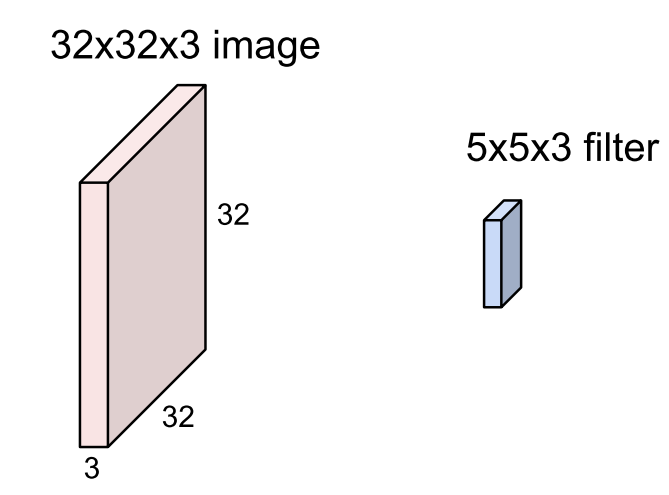
\includegraphics[width=.4\textwidth]{convlayer.png}
	\label{fig:convlayer}
	\caption{Example of convolutional Layer(with one filter)}
\end{figure}

Pooling layers are sometime used right after Conv-ReLU layers to squeeze the spatial size(height and width) of flowing tensors to lower the number of learnable weights of the remaining layers. 
\begin{figure}[H]
	\centering
	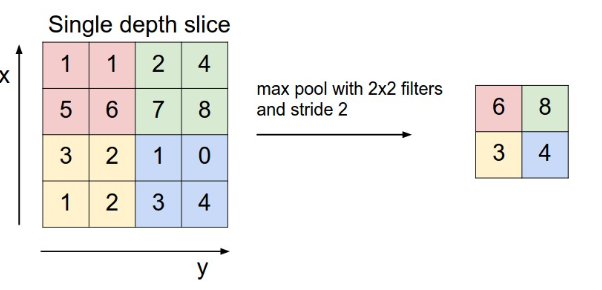
\includegraphics[width=.5\textwidth]{poolinglayer.png}
	\label{fig:poolinglayer}
	\caption{Example of pooling layer}
\end{figure}

The course listed some famous CNN architectures like AlexNet, VGGNet, GoogLeNet and ResNet, all of which are ImageNet competitions' winners. It then compared the space of memory that the models used and number of weight parameters in each layers among those models, which made a good exercise to break down the models in more detail.


\section{Recurrent Neural Networks and Long Short-Term Memories}
%RNNs are more capable of processing sequential input data like conversations and sentences than CNNs. But vanilla RNNs suffer lot from gradient vanishing problems. LSTMs design complex cells that help preserving the error that can be backpropagated through time and layers. So LSTMs are widely used to do tasks like image captioning and machine translation.

\paragraph{RNN}
Unlike feed forward neural networks, recurrent neural networks take as their input not just the current input example they see, but also what they have perceived previously in time. The decision a recurrent net reached at time step $t-1$ affects the decision it will reach one moment later at time step $t$. So RNNs have two sources of input, the present and the recent past. The sequential information is preserved in the recurrent network’s hidden state, which manages to span many time steps as it cascades forward to affect the processing of each new example. One way to think about RNNs is this: they are a way to share weights over time. Therefore RNNs are good at processing sequences like image caption and machine translation. 

\begin{figure}[H]
	\centering
	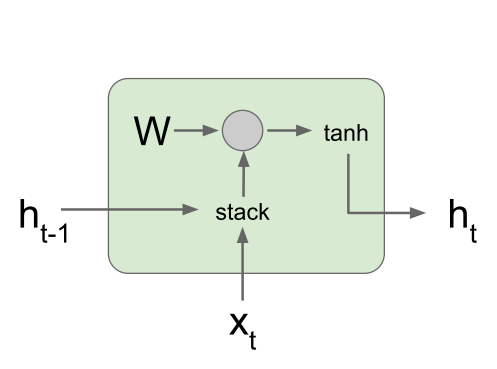
\includegraphics[width=.4\textwidth]{rnn-unit.png}
	\caption{RNN unit}
\end{figure}

The forward pass of a RNN block can be mathematically described as:
\begin{equation}
h_t=f_W(h_{t-1},x_t)=W_h^T \cdot h_{t-1} + W_x^T \cdot x_t
\label{eqn:rnn}
\end{equation}

where $h_t$ is the current hidden state at time step $t$; $f_W$ the function -- either sigmoid or tanh -- that squashes the sum of the weight input and hidden state,  making gradients workable for backpropagation; $h_{t-1}$ the previous hidden state; $x_t$ the input at the same time step.

Recurrent networks rely on an extension of backpropagation called backpropagation through time, or BPTT. Time, in this case, is simply expressed by a well-defined, ordered series of calculations linking one time step to the next, which is all backpropagation needs to work.

However, RNNs suffer a lot from vanishing/exploding gradient problems. Intuitively, backpropagation from $h_t$ to $h_{t-1}$ multiplies by $W_h$, so computing gradient of $h_0$ involves many factors of $W_h$. If the largest singular value of $W_h$ is greater than $1$, then exploding gradients would occur; on the contrary if the largest singular value of $W_h$ if less than $1$, then vanishing gradients would happen. Exploding gradients can be solved relatively easily, because they can be truncated or squashed. Vanishing gradients can become too small for computers to work with or for networks to learn – a harder problem to solve. 

\paragraph{LSTM}
Long short-term memory was proposed to solve vanishing gradient problem of vanilla RNNs. LSTMs design complicated cells that help preserve the error that can be backpropagated through time and layers.

\begin{figure}[H]
	\centering
	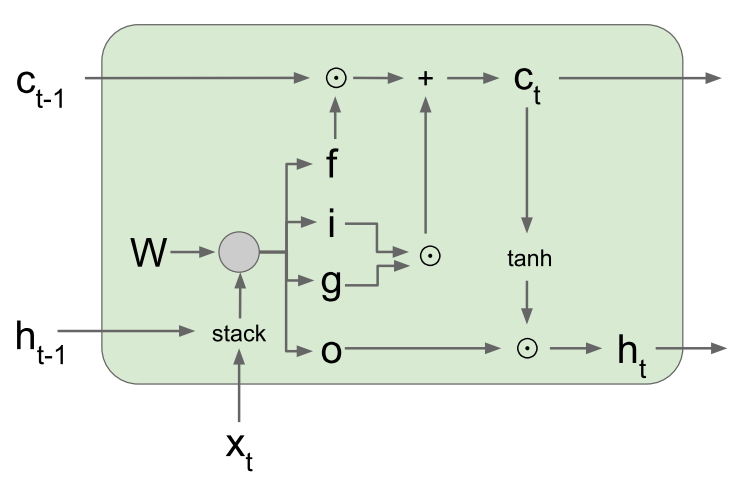
\includegraphics[width=.6\textwidth]{lstm-cell.png}
	\caption{LSTM cell}
\end{figure}

The forward pass of a LSTM cell is defined as follows:
\begin{equation}
\begin{split}
\left(\begin{array}{c} i\\f\\o\\g \end{array}\right) &= \left(\begin{array}{c} \sigma\\\sigma\\\sigma\\\tanh \end{array}\right) W \left(\begin{array}{c} h_{t_1}\\x_t \end{array}\right)  \\  
c_t &= f \odot c_{t_1} + i \odot g\\
h_t &= o \odot \tanh(c_t)
\end{split}
\label{eqn:lstm}
\end{equation}
where $\odot$ is element-wise multiplication.

As described in equation \ref{eqn:lstm}, all the computations involved, including sigmoid,  element-wise multiplication and so on, are differentiable, which are suitable for backpropagation. 

Those gates act on the signals they receive, and similar to the neural network’s nodes, they block or pass on information based on its strength and input, which they filter with their own sets of weights. Those weights, like the weights that modulate input and hidden states, are adjusted via the recurrent networks learning process. That is, the cells learn when to allow data to enter, leave or be deleted through the iterative process of making guesses, backpropagating error, and adjusting weights via gradient descent.


\section{Generative Models}
%Generative models focus on modeling class-conditional probabilistic distribution functions and prior probabilities, and a good outcome is that generative models can generate synthetic data points. Therefore generative adversarial networks become an active research field in the last few years due to this feature.

Neural network models we have learned so far, such as feed forward networks, CNNs, RNNs, LSTMs, are all basically discriminative models, which directly estimate posterior probabilities. Generative models focus on modeling class-conditional probabilistic distribution functions and prior probabilities with a good outcome that generative models can generate synthetic data points. Therefore generative adversarial networks become an active research field in the last few years due to this feature. 

CS231 course discussed generative models like PixelRNN, PixelCNN, variational autoencoder and generative adversarial networks, and used them to generate instances or do other interesting tasks. 

GAN consists of generator network and discriminator network. The generator network tries to fool the discriminator by generating real-looking images from random noise, while discriminator network tries to distinguish between real and fake images. These two networks are trained jointly in minmax game. The minmax objective function is defined as follows:
$$\min_{\theta_g} \max_{\theta_d}\left[\mathbb{E}_{x \sim p_{data}} \log D_{\theta_d}(x) + \mathbb{E}_{z \sim p(z)} \log(1-D_{\theta_d}(G_{\theta_g}(z)))\right]$$

Training this minmax objective function can be separated apart as two functions:
\begin{enumerate}
	\item Gradient ascent on discriminator
		\begin{equation*}
		\max_{\theta_d}\left[\mathbb{E}_{x \sim p_{data}} \log D_{\theta_d}(x) + \mathbb{E}_{z \sim p(z)} \log(1-D_{\theta_d}(G_{\theta_g}(z)))\right]
		\end{equation*}
	\item Gradient descent on generator
		\begin{equation}		
		\min_{\theta_g}\mathbb{E}_{z \sim p(z)}\log(1-D_{\theta_d}(G_{\theta_g}(z)))
		\label{eqn:generator-gd}
		\end{equation}
\end{enumerate}

However in practice optimizing generator objective does not work well because when sample is likely fake, we want to learn from it to improve generator, but gradient of function $\log(1-x)$ near $x=0$ is relatively flat. Therefore instead of minimizing likelihood of discriminator being correct(see equation\ref{eqn:generator-gd}), now maximize likelihood of discriminator being wrong(see equation\ref{eqn:generator-ga}). It's the same objective of fooling discriminator, but now there is higher gradient signal for bad samples so that it works much better.

\begin{enumerate}
	\item Gradient ascent on discriminator
	\begin{equation}
	\max_{\theta_d}\left[\mathbb{E}_{x \sim p_{data}} \log D_{\theta_d}(x) + \mathbb{E}_{z \sim p(z)} \log(1-D_{\theta_d}(G_{\theta_g}(z)))\right]
	\label{eqn:discriminator-ga}
	\end{equation}
	\item Gradient ascent on generator
	\begin{equation}		
	\max_{\theta_g}\mathbb{E}_{z \sim p(z)}\log(D_{\theta_d}(G_{\theta_g}(z)))
	\label{eqn:generator-ga}
	\end{equation}
\end{enumerate}

In the experiment these two objectives(equation \ref{eqn:discriminator-ga} and \ref{eqn:generator-ga}) are negated as we will be minimizing these losses. More implementation details are covered in section \ref{sec:assignment3-gan}.

\section{Assignment 1}
Assignment 1 requires us to implement KNN algorithm, SVM and softmax classifier.
\subsection{KNN}
In this part KNN is implemented with two loops, one loop and fully vectorized. KNN with two loops is naive and a nested for-loop will do. The one loop version just iterates test data, and computes the distances between this data and all the training data, with the help of broadcast feature of numpy.
\begin{lstlisting}
for i in range(num_test):
	dists[i, :] = np.sqrt(np.sum((X[i, :] - self.X_train)**2, axis=1))
return dists
\end{lstlisting}

These two versions are not so difficult, but the no loop version demands full vectorized computation, which makes it much trickier to implement. To be honest I didn't figure it out, so I had to search the Internet and then found the solution, which makes good use of broadcast feature of numpy. The code is as follows:
\begin{lstlisting}[language=python]
P = np.sum(X**2, axis=1)
Q = np.sum(self.X_train**2, axis=1)
PQ = X.dot(self.X_train.T)
dists = np.sqrt(np.transpose([P]) + Q - 2*PQ)
\end{lstlisting}
Let $p$ denotes test data matrix, $q$ training data matrix, and $dist$ distance matrix. The equation of distance is $(p-q)^2$. There is no way to just simple subtract test and training data and square the subtraction because they don't have the same shape. However, the solution applies the equation $(p\pm q)^2=p^2 \pm 2pq + q^2$, and the term $p^2$ and $q^2$ are easy to vectorize, the middle term $2pq$ is dot multiplication of two matrix, so it is also vectorized. But actually these three terms have totally different shapes. In code line 1 above, $P$ has shape (num\_test,) --- which in numpy indicates that this array has 1 dimension with size num\_test. Similarly, $Q$ has shape (num\_train,), and $PQ$ has shape (num\_test, num\_train). Here is the trick. if we compute $[P].T-Q$ instead, these two array will be broadcast, and yields result with shape (num\_test, num\_train).

The assignment then compare the time cost among these three versions of implementation. The result shows marvelous improvement that vectorization does.
\begin{table}[h]
	\centering
	\begin{tabular}{c|c|c}
		\hline
		two loops & one loop & no loops\\
		\hline
		36.73 & 121.6 & 0.33\\
		\hline
	\end{tabular}
	\caption{Comparing KNN Performance}
\end{table}

The assignment also compares the influence of different Ks.
\begin{figure}[h]
	\centering
	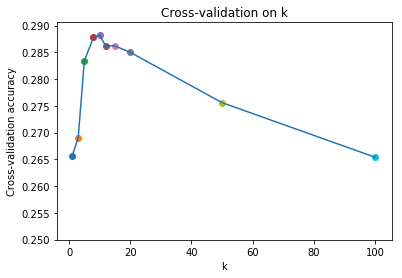
\includegraphics[width=.5\textwidth]{knn-k.png}
\end{figure}

\subsection{SVM, Softmax and Two layer Neural Network}
The assignment compares the accuracy tested on CIFAR-10 dataset among linear SVM, softmax, and two layer neural network with L2 regularization.
\begin{table}[H]
	\centering
	\begin{tabular}{c|c|c|c}
		\hline
		& SVM & softmax & NN\\
		\hline
		accuracy & 0.377 & 0.357 & 0.494\\
		\hline
	\end{tabular}
\end{table}
We can see that a simple two layer neural network can easily exceed SVM and softmax by 10 more percentage.


\section{Assignment 2}
Assignment 2 requires us to implement fully connected neural network and convolutional neural network in modular style and batch normalization layer.

\subsection{Fully Connected Neural Network}
In assignment 1 a fully-connected two-layer neural network is implemented on CIFAR-10. The implementation is simple but not very modular since the loss and gradient are computed in a single monolithic function. This is manageable for a simple two-layer network, but would become impractical as we move to bigger models.

Then it compares different update rules like vanilla SGD, SGD with momentum, Adam and RMSProp. The results shows that vanilla SGD is worse than all the other more sophisticated ones on both speed and accuracy.
\begin{figure}[h]
	\centering
	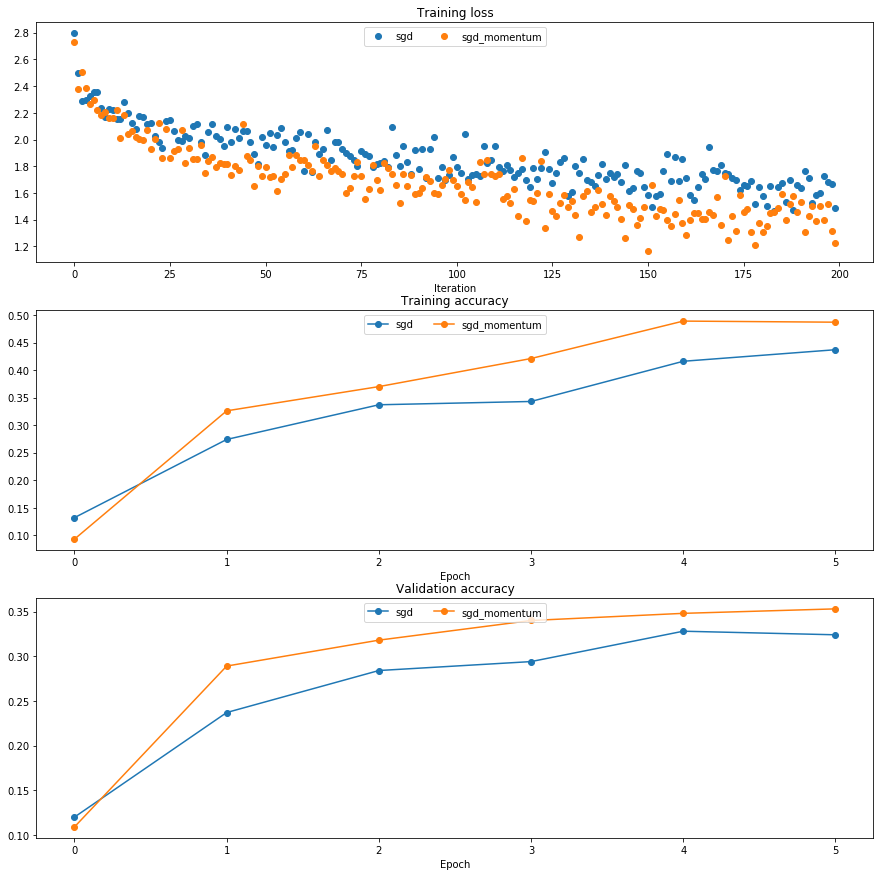
\includegraphics[width=.8\textwidth]{update-rules.png}
	\caption{Comparing update rules}
\end{figure}

\subsection{Batch Normalization}
Figure \ref{img:bn-convergence} shows that batch normalization helps models to converge much faster.
\begin{figure}[htbp]
	\centering
	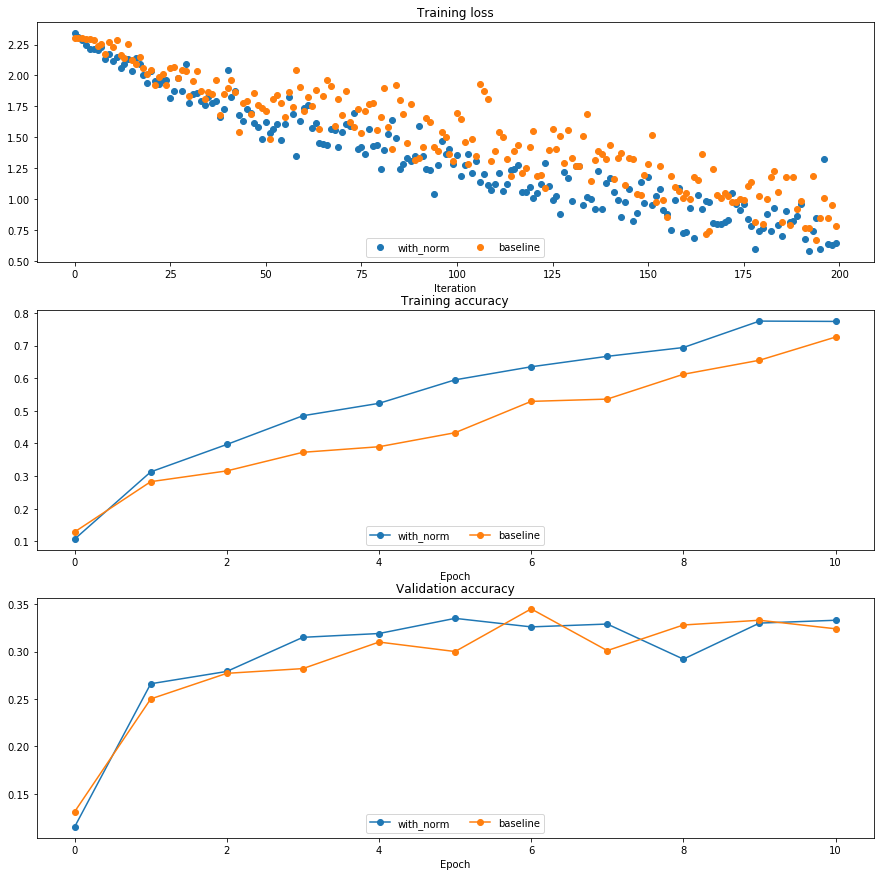
\includegraphics[width=.7\textwidth]{bn-acc.png}
	\caption{Batch Normalization helps model to converge faster.}
	\label{img:bn-convergence}
\end{figure}

Besides, as represented in figure \ref{img:bn-init}, using batch normalization can make network less sensitive the the scale of weight initialization and therefore make it more stable.
\begin{figure}[htbp]
	\centering
	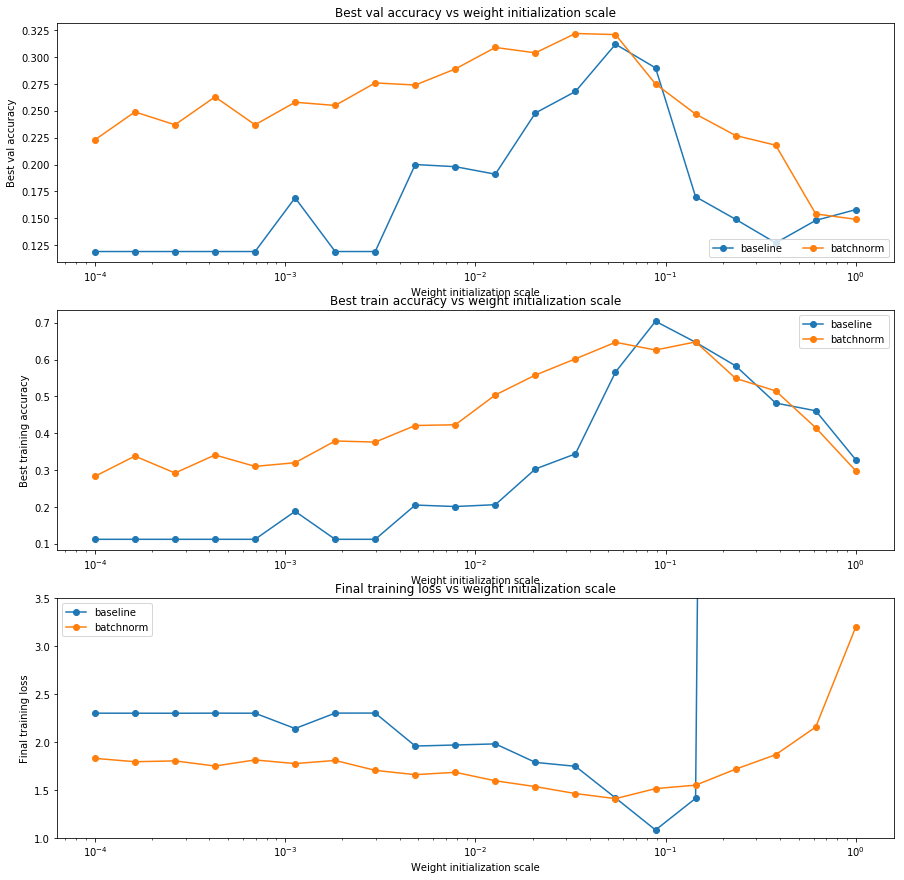
\includegraphics[width=.7\textwidth]{bn-init.png}
	\caption{Batch normalization makes model more stable.}
	\label{img:bn-init}
\end{figure}

The forward pass of batch normalization layer is easy to write codes, but the lecture doesn't derive the backward pass so I have to do it on my own. The naive backward pass can be further simplified because some internal variables are unnecessary to compute the final results. And the experiment shows that the simplified version is twice faster than naive one.

\subsection{Convolutional Neural Network}
The lecture doesn't talk much about the backpropagation of convolutional layer either. I didn't figure out how to derive it in the beginning so I searched some blogs and tutorials. But luckily I understood how to derive the gradients of convolutional layer in the end. 

In the final part of assignments we are asked to train a model with whatever ConvNet architecture on CIFAR-10 and achieve at least 70\% accuracy on the CIFAR-10 validation set within 10 epochs.

The default setting(3-layered ConvNet) achieves 50\% accuracy, so there is a long way to go. First I tune the learning rate to find the optimal result. It turns out that setting learning rate to be 1.8e-3 will increase the accuracy to 59.8\%. Then I insert batch normalization layers after each convolutional layer and stack more convolutional layers(6 conv layers in total), and all kernels have size $3\times 3$. At the same time I set every two conv layers striding 2 instead of 1 to perform as dropout. The final 7-layered ConvNet trained in 10 epochs easily achieves 74.86\% accuracy on validation set, outperforming the baseline by 4.86\%. The model also has 74.8\% accuracy on test set, showing that there is little overfitting problem.


\section{Assignment 3}
Assignment 3 requires us to implement image captioning with RNN and LSTM, style transfer, network visualization and GAN.

\subsection{Image Captioning with RNN and LSTM}
Implementing RNN and LSTM cells are not difficult because all the functions inside are basic and differentiable. In this part I implemented image captioning with a single RNN/LSTM cell, which turns out that they both can fit the training set but behave somewhat bad on validation set(shown in Figure \ref{fig:side:a} and \ref{fig:side:b}).
\begin{figure}
\begin{minipage}[t]{0.5\textwidth}
	\centering
	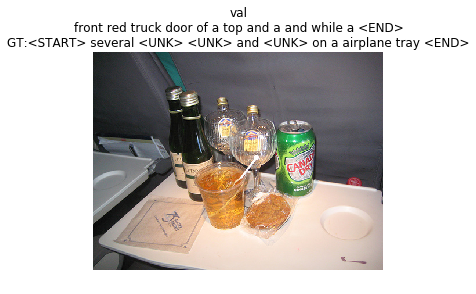
\includegraphics[width=\textwidth]{rnn-caption.png}
	\caption{Image captioning with RNN}
	\label{fig:side:a}
\end{minipage}%
\begin{minipage}[t]{0.5\textwidth}
	\centering
	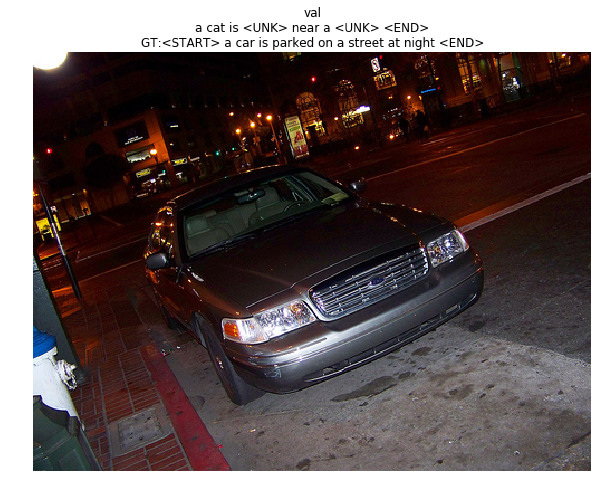
\includegraphics[width=.8\textwidth]{lstm-caption.png}
	\caption{Image captioning with LSTM}
	\label{fig:side:b}
\end{minipage}
\end{figure}

\subsection{Network Visualization}
A saliency map tells us the degree to which each pixel in the image affects the classification score for that image. In this experiment we use pre-trained SqueezeNet to compute the scores given input image, and then compute gradients with respect to each pixels rather than parameters as we do in discriminative models. Figure \ref{fig:saliency-map} shows almost accurate saliency map of the given images and classes.
\begin{figure}[htbp]
	\centering
	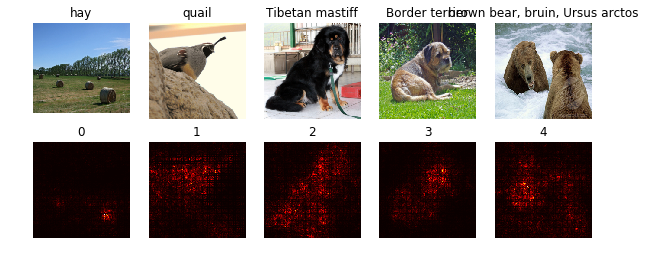
\includegraphics[width=.7\textwidth]{saliency.png}
	\caption{Saliency Map}
	\label{fig:saliency-map}
\end{figure}

\subsection{Generative Adversarial Networks} \label{sec:assignment3-gan}
In a GAN, we build two different neural networks. Our first network is a traditional classification network, called the discriminator. We will train the discriminator to take images, and classify them as being real (belonging to the training set) or fake (not present in the training set). Our other network, called the generator, will take random noise as input and transform it using a neural network to produce images. The goal of the generator is to fool the discriminator into thinking the images it produced are real.

\paragraph{Original GAN} In this experiment we alter the loss function as well as architecture of discriminator and generator of GAN. In the original GAN, we use fully-connected discriminator and generator, and the generator loss and discriminator loss are as follows:
\begin{eqnarray*}
	\ell_G  &=&  -\mathbb{E}_{z \sim p(z)}\left[\log D(G(z))\right]\\
	\ell_D &=& -\mathbb{E}_{x \sim p_\text{data}}\left[\log D(x)\right] - \mathbb{E}_{z \sim p(z)}\left[\log \left(1-D(G(z))\right)\right]
\end{eqnarray*}

And we use binary cross entropy loss to compute the log probability of the true label given the logits output from the discriminator. Given a score $s\in\mathbb{R}$ and a label $y\in\{0, 1\}$, the binary cross entropy loss is
$$ bce(s, y) = -y * \log(s) - (1 - y) * \log(1 - s) $$

Figure \ref{fig:gan-origin} shows what it can generate after 3000+ iterations of training. Most of them have random noises and are hard to recognize for human.

\paragraph{LSGAN} Least squares GAN alter the loss functions of discriminator and generator to make it more stable. 
\begin{eqnarray*}
\ell_G &=&  \frac{1}{2}\mathbb{E}_{z \sim p(z)}\left[\left(D(G(z))-1\right)^2\right]\\
\ell_D &=& \frac{1}{2}\mathbb{E}_{x \sim p_\text{data}}\left[\left(D(x)-1\right)^2\right] + \frac{1}{2}\mathbb{E}_{z \sim p(z)}\left[ \left(D(G(z))\right)^2\right]
\end{eqnarray*}

Figure \ref{fig:ls-origin} shows that the results are slightly better than the original GAN because most of them are recognizable, but still have some random noises.

\paragraph{DCGAN} Deeply convolutional GANs use CNN in their discriminator and generator. The results shown in Figure \ref{fig:dc-origin} are pretty clear and without any random noise.
\begin{figure}[htbp]
	\begin{minipage}[t]{0.33\textwidth}
		\centering
		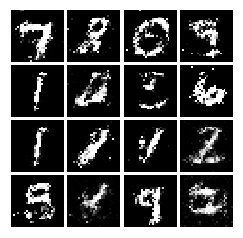
\includegraphics[width=\textwidth]{gan-origin.png}
		\caption{Original GAN}
		\label{fig:gan-origin}
	\end{minipage}
	\begin{minipage}[t]{.33\textwidth}
		\centering
		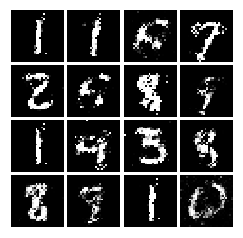
\includegraphics[width=\textwidth]{ls-gan.png}
		\caption{LSGAN}
		\label{fig:ls-origin}
	\end{minipage}
	\begin{minipage}[t]{.33\textwidth}
		\centering
		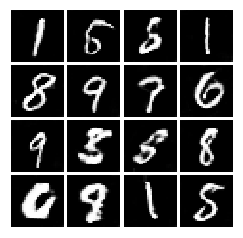
\includegraphics[width=\textwidth]{dc-gan.png}
		\caption{DCGAN}
		\label{fig:dc-origin}
	\end{minipage}
\end{figure}


\section{Conclusion}
This course is a deep dive into details of the deep learning architectures with a focus on learning end-to-end models for visual recognition tasks, particularly image classification. From the course I learned to implement, train and debug my own neural network models and gained a detailed understanding of cutting-edge research in computer vision. 

\end{document}
